\documentclass[a4paper,12pt]{report} 


\usepackage[francais]{babel}

\usepackage[T1]{fontenc} 
\usepackage[utf8]{inputenc} 
\usepackage{lmodern} 
\usepackage{color} 
\usepackage{graphicx} 
  
\usepackage{hyperref}
\hypersetup{
    colorlinks,
    citecolor=black,
    filecolor=black,
    linkcolor=black,
    urlcolor=black
}

\usepackage{listings}
\usepackage{color}
\usepackage{placeins}


  

\author{ 
\textit{CHASAN Lucie}\\
\textit{ESCURE Florian}\\
\textit{MATHE Lucie}\\
\textit{MONTERO Eliott}\\
}   
\title{\textbf{Compte rendu TD 1 Projet de Programmation}} 
\date{23 Janvier 2019}
  

\begin{document}
\begin{figure}[!b] 
\begin{center} 
\href{Copyright 1994 David Farley}{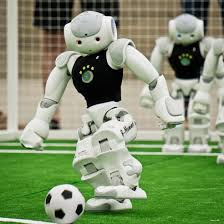
\includegraphics[scale = 1]{robocup.jpg}}
\end{center} 
\end{figure} 
  
\maketitle

\newpage

Lors de notre premier TD avec notre chargé de TD, M. Philippe NARBEL, nous avons d'abord vu l'introduction du fonctionnement du TD, de comment il va nous aiguiller et nous aider à nous concentrer sur les tâches les plus importantes.
\newline
Nous devons push une ébauche basique du code testé (méthodes openCV) et du cahier des besoins pour mardi soir environ.
\newline
Il a été souligné que plus nous donnons d'informations le plus tôt possible à notre chargé de TD, le mieux ce serait pour qu'il comprenne où nous y sommes, de plus nous avons eu d'autres conseils sur comment gérer le projet :
\begin{itemize}
    \item Il est préférable de garder les documents prototypes (Code non-utilisés dans le projet final, rapports de progression comme celui-ci, etc) dans le git, car ils peuvent être utiles en tant qu'annexe.
    \item Il est important de bien définir une version basique et réalisable, pour se donner un objectif à atteindre relativement rapidement et à s'y tenir.
    \item Il faut faire attention à ne pas être confus à cause d'un grand nombre de besoins non fonctionnels, on doit d'abord se concentrer sur la création d'une base fonctionnelle, la suite viendra après.
    \item Attention aux jeux de données, comme nous avons beaucoup de matière à travailler il faut bien penser aux tests, comme demander des vidéos aux clients dans des conditions plus favorables que celles que nous avons déjà.
    \item Bien se renseigner sur OpenCV et les méthodes utilisables pour notre situation
\end{itemize}

\newline
Nous avons aussi principalement parlé du principe de notre projet et expliqué son fonctionnement à notre chargé de TD.

\end{document}
